% Standalone vector figure. Rebuild with: bash docs/build-short-paper.sh
\documentclass[tikz,border=5pt]{standalone}
\usepackage[T1]{fontenc}
\usepackage{lmodern}
\usetikzlibrary{arrows.meta,calc,backgrounds}

\definecolor{ink}{HTML}{223449}
\definecolor{muted}{HTML}{536779}
\definecolor{research}{HTML}{926124}
\definecolor{researchbg}{HTML}{FCF7EE}
\definecolor{core}{HTML}{246775}
\definecolor{corebg}{HTML}{F0F7F8}
\definecolor{view}{HTML}{495FA0}
\definecolor{viewbg}{HTML}{F3F5FC}
\definecolor{rule}{HTML}{CCD6DF}

\begin{document}
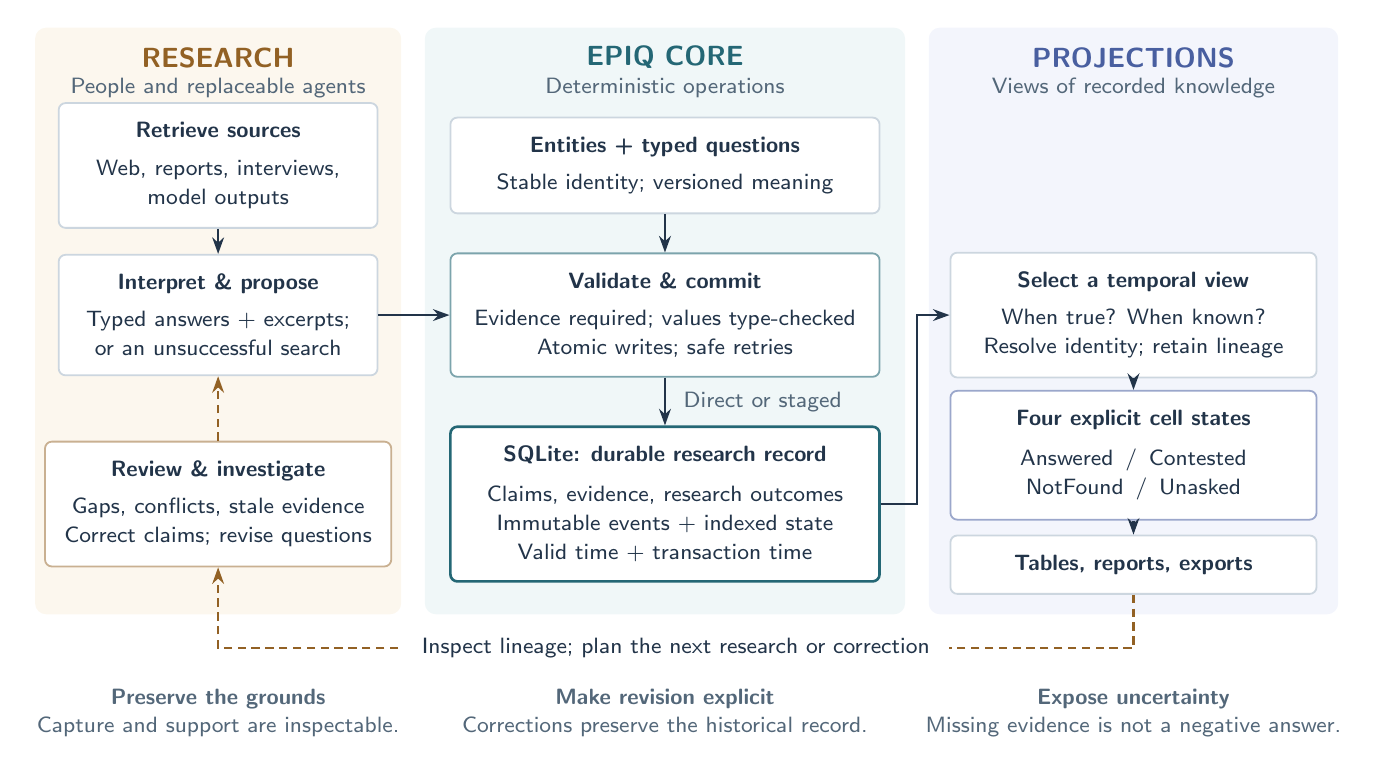
\begin{tikzpicture}[
  x=1cm,y=1cm,
  font=\sffamily\fontsize{8.5}{10.5}\selectfont,
  text=ink,
  box/.style={draw=rule,line width=.65pt,rounded corners=2.5pt,
    fill=white,align=center,inner sep=7pt},
  heading/.style={font=\sffamily\bfseries\fontsize{10}{12}\selectfont},
  detail/.style={font=\sffamily\fontsize{8}{10}\selectfont,text=muted},
  flow/.style={-{Stealth[length=2.1mm,width=1.5mm]},line width=.85pt,draw=ink},
  feedback/.style={-{Stealth[length=2.1mm,width=1.5mm]},line width=.85pt,
    draw=research,dash pattern=on 3pt off 2pt},
]

% Three lanes separate fallible research, deterministic storage, and views.
\fill[researchbg,rounded corners=4pt] (0,0) rectangle (4.65,-7.45);
\fill[corebg,rounded corners=4pt] (4.95,0) rectangle (11.05,-7.45);
\fill[viewbg,rounded corners=4pt] (11.35,0) rectangle (16.55,-7.45);

\node[heading,text=research] at (2.325,-.38) {RESEARCH};
\node[detail] at (2.325,-.76) {People and replaceable agents};
\node[heading,text=core] at (8,-.38) {EPIQ CORE};
\node[detail] at (8,-.76) {Deterministic operations};
\node[heading,text=view] at (13.95,-.38) {PROJECTIONS};
\node[detail] at (13.95,-.76) {Views of recorded knowledge};

\node[box,minimum width=4.05cm,minimum height=1.12cm] (sources) at (2.325,-1.75)
  {\textbf{Retrieve sources}\\[3pt]
   Web, reports, interviews,\\model outputs};
\node[box,minimum width=4.05cm,minimum height=1.3cm] (interpret) at (2.325,-3.65)
  {\textbf{Interpret \& propose}\\[3pt]
   Typed answers + excerpts;\\or an unsuccessful search};
\node[box,draw=research!50,minimum width=4.05cm,minimum height=1.35cm] (review) at (2.325,-6.05)
  {\textbf{Review \& investigate}\\[3pt]
   Gaps, conflicts, stale evidence\\Correct claims; revise questions};

\node[box,minimum width=5.45cm,minimum height=1.12cm] (schema) at (8,-1.75)
  {\textbf{Entities + typed questions}\\[3pt]
   Stable identity; versioned meaning};
\node[box,draw=core!60,minimum width=5.45cm,minimum height=1.3cm] (validate) at (8,-3.65)
  {\textbf{Validate \& commit}\\[3pt]
   Evidence required; values type-checked\\Atomic writes; safe retries};
\node[box,draw=core,line width=.95pt,minimum width=5.45cm,minimum height=1.5cm] (store) at (8,-6.05)
  {\textbf{SQLite: durable research record}\\[4pt]
   Claims, evidence, research outcomes\\Immutable events + indexed state\\Valid time + transaction time};

\node[box,minimum width=4.65cm,minimum height=1.3cm] (project) at (13.95,-3.65)
  {\textbf{Select a temporal view}\\[3pt]
   When true? When known?\\Resolve identity; retain lineage};
\node[box,draw=view!55,minimum width=4.65cm,minimum height=1.05cm] (states) at (13.95,-5.43)
  {\textbf{Four explicit cell states}\\[4pt]
   Answered\enspace /\enspace Contested\\NotFound\enspace /\enspace Unasked};
\node[box,minimum width=4.65cm,minimum height=.72cm] (outputs) at (13.95,-6.82)
  {\textbf{Tables, reports, exports}};

\draw[flow] (sources) -- (interpret);
\draw[flow] (interpret.east) -- (validate.west);
\draw[flow] (schema) -- (validate);
\draw[flow] (validate) -- node[right,detail,align=left,xshift=3pt]
  {Direct or staged} (store);
\draw[flow] (store.east) -- (11.2,-6.05) -- (11.2,-3.65) -- (project.west);
\draw[flow] (project) -- (states);
\draw[flow] (states) -- (outputs);

% Feedback is a new research action, never a silent rewrite of prior evidence.
\draw[feedback] (outputs.south) -- (13.95,-7.88) --
  node[midway,fill=white,inner xsep=7pt,inner ysep=3pt,
       font=\sffamily\fontsize{8}{10}\selectfont]
  {Inspect lineage; plan the next research or correction} (2.325,-7.88)
  -- (review.south);
\draw[feedback] (review.north) -- (interpret.south);

% Short invariants make the diagram readable without the surrounding paper.
\node[detail,align=center] at (2.325,-8.7)
  {\textbf{Preserve the grounds}\\Capture and support are inspectable.};
\node[detail,align=center] at (8,-8.7)
  {\textbf{Make revision explicit}\\Corrections preserve the historical record.};
\node[detail,align=center] at (13.95,-8.7)
  {\textbf{Expose uncertainty}\\Missing evidence is not a negative answer.};
\end{tikzpicture}
\end{document}
